\chapter{Desarrollo}
Este proyecto se desarrollará con la metodología SCRUM con 8 sprints de una revision por semana, haciendo uso de historias de usuario y de la grafica del quemado para llevar un control de que historias de usuario se quemaron.

\section{Recursos}
\subsection{Recursos humanos}
\begin{table}[H]
\centering
\begin{tabular}{|l|l|l|}
\hline
Rol               & Personas requeridas & Salario  \\ \hline
Programador       & 1                   & \$15,000 \\ \hline
Diseñador         & 1                   & \$10,000 \\ \hline
Tester            & 1                   & \$10,000 \\ \hline
Lider de proyecto & 1                   & \$15,000 \\ \hline
\end{tabular}
\caption{Tabla del pesonal requerido.}
\label{personal}
\end{table}

\subsection{Recursos materiales}
\begin{table}[H]
\centering
\begin{tabular}{|l|l|l|}
\hline
Equipo          & Precio  & Unidades necesarias \\ \hline
Computadoras    & \$8,000 & 2                   \\ \hline
Celular Android & \$5,000 & 1                   \\ \hline
\end{tabular}
\caption{Tabla de recursos materiales.}
\label{materiales}
\end{table}

\subsection{Recursos tecnológicos}
\begin{table}[H]
\centering
\begin{tabular}{|l|l|}
\hline
Concepto       & Precio  \\ \hline
GanttProject   & \$0 \\ \hline
Pencil         & \$0 \\ \hline
Android Studio & \$0 \\ \hline
\end{tabular}
\caption{Tabla de recursos tecnológicos}
\label{tecnologicos}
\end{table}

\subsection{Recursos administrativos}
\begin{table}[H]
\centering
\begin{tabular}{|l|l|}
\hline
Concepto     & Precio       \\ \hline
Agua         & \$100 al mes \\ \hline
Electricidad & \$300 al mes \\ \hline
Internet     & \$500 al mes \\ \hline
\end{tabular}
\caption{Tabla de recursos administrativos}
\label{administrativos}
\end{table}

\section{Diagrama de Gantt}
\begin{figure}[H]
	\begin{center}
		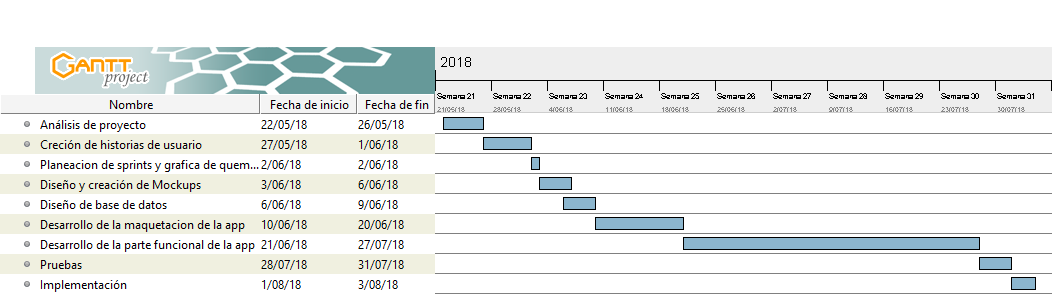
\includegraphics[scale=0.6]{img/cronograma.png} 
		\caption{Cronograma de actividades a seguir.}
		\label{gantt}
	\end{center}
\end{figure}

\section{Historias de usuario}

\begin{table}[H]\small
\begin{tabular}{@{\extracolsep{\fill}} | p{5cm} | p{5cm} | p{5cm} | }
\multicolumn{3}{|c|}{1. Aplicación didactica} \\ \hline
  \hline
\multicolumn{3}{|p{15cm}|}{Como usuario quisiera que la aplicación fuera de un modo didáctica y de aprendizaje mediante ejercicios.} \\ \hline
\hline
Estimaci'on: 7 &semanas	Valor: 50	& Dependencias: \\
\hline
\multicolumn{3}{|p{15cm}|}{Condiciones de satisfacci'on:
\begin{itemize}
	\item La aplicación contendrá información selecta y bien explicada.
	\item Se incluirán algunos ejercicios los cuales deberán resolverse en la computadora.
\end{itemize}
}\\ \hline
\hline
\end{tabular}
\caption{Historia de usuario 1}
\label{hu1}
\end{table}
%%%%%%%%%%%%%%%%%%%%%%%%%%%%%%%%%%%%%%%%%%%%%%%%%%%%%%%%%%%%%%%%%%%%%%%%%%%%%%%%%%%%%%
\begin{table}[H]\small
\begin{tabular}{@{\extracolsep{\fill}} | p{5cm} | p{5cm} | p{5cm} | }
\multicolumn{3}{|c|}{2. Explicaciónes detalladas} \\ \hline
  \hline
\multicolumn{3}{|p{15cm}|}{Como usuario quisiera que explicara a detalle cómo hacer las cosas y para que podrían servir.} \\ \hline
\hline
Estimaci'on: 7 &semanas	Valor: 60	& Dependencias: \\
\hline
\multicolumn{3}{|p{15cm}|}{Condiciones de satisfacci'on:
\begin{itemize}
	\item Se dará una aplicación detallada de cada tema así como ejemplos de uso.
\end{itemize}
}\\ \hline
\hline
\end{tabular}
\caption{Historia de usuario 2}
\label{hu2}
\end{table}
%%%%%%%%%%%%%%%%%%%%%%%%%%%%%%%%%%%%%%%%%%%%%%%%%%%%%%%%%%%%%%%%%%%%%%%%%%%%%%%%%%%%%%
\begin{table}[H]\small
\begin{tabular}{@{\extracolsep{\fill}} | p{5cm} | p{5cm} | p{5cm} | }
\multicolumn{3}{|c|}{3. Modalidad de juegos} \\ \hline
  \hline
\multicolumn{3}{|p{15cm}|}{Como usuario quisiera que la aplicación tuviera la modalidad de juegos, con breves capsulas que expliquen la teoría.} \\ \hline
\hline
Estimaci'on: 6 &semanas	Valor: 60	& Dependencias: \\
\hline
\multicolumn{3}{|p{15cm}|}{Condiciones de satisfacci'on:
\begin{itemize}
	\item Se pondrá información sobre algunos conceptos y se hará un pequeño test de manera que ayude a recordar.
\end{itemize}
}\\ \hline
\hline
\end{tabular}
\caption{Historia de usuario 3}
\label{hu3}
\end{table}
%%%%%%%%%%%%%%%%%%%%%%%%%%%%%%%%%%%%%%%%%%%%%%%%%%%%%%%%%%%%%%%%%%%%%%%%%%%%%%%%%%%%%%
\begin{table}[H]\small
\begin{tabular}{@{\extracolsep{\fill}} | p{5cm} | p{5cm} | p{5cm} | }
\multicolumn{3}{|c|}{4. Información especifica} \\ \hline
  \hline
\multicolumn{3}{|p{15cm}|}{Como usuario quisiera que tuviera información específica del tema y vídeos tutoriales para poder facilitar la comprensión de los temas.} \\ \hline
\hline
Estimaci'on: 6 &semanas	Valor: 30	& Dependencias: \\
\hline
\multicolumn{3}{|p{15cm}|}{Condiciones de satisfacci'on:
\begin{itemize}
	\item Se dará la información de manera específica pero en lugar de videos se incluirán algunos ejemplos.
\end{itemize}
}\\ \hline
\hline
\end{tabular}
\caption{Historia de usuario 4}
\label{hu4}
\end{table}
%%%%%%%%%%%%%%%%%%%%%%%%%%%%%%%%%%%%%%%%%%%%%%%%%%%%%%%%%%%%%%%%%%%%%%%%%%%%%%%%%%%%%%
\begin{table}[H]\small
\begin{tabular}{@{\extracolsep{\fill}} | p{5cm} | p{5cm} | p{5cm} | }
\multicolumn{3}{|c|}{5. Visual y practica} \\ \hline
  \hline
\multicolumn{3}{|p{15cm}|}{Como usuario quisiera que la aplicación fuera visual y práctica.} \\ \hline
\hline
Estimaci'on: 4 &semanas	Valor: 20	& Dependencias: \\
\hline
\multicolumn{3}{|p{15cm}|}{Condiciones de satisfacci'on:
\begin{itemize}
	\item La aplicación será visual y de fácil utilización.
\end{itemize}
}\\ \hline
\hline
\end{tabular}
\caption{Historia de usuario 5}
\label{hu5}
\end{table}
%%%%%%%%%%%%%%%%%%%%%%%%%%%%%%%%%%%%%%%%%%%%%%%%%%%%%%%%%%%%%%%%%%%%%%%%%%%%%%%%%%%%%%
\begin{table}[H]\small
\begin{tabular}{@{\extracolsep{\fill}} | p{5cm} | p{5cm} | p{5cm} | }
\multicolumn{3}{|c|}{6. Intuitiva} \\ \hline
  \hline
\multicolumn{3}{|p{15cm}|}{Como usuario quisiera que la aplicación fuera intuitiva y con muchos ejercicios.} \\ \hline
\hline
Estimaci'on: 3 &semanas	Valor: 20	& Dependencias: \\
\hline
\multicolumn{3}{|p{15cm}|}{Condiciones de satisfacci'on:
\begin{itemize}
	\item Se creará una interfaz amigable con el usuario y fácil de aprender.
\end{itemize}
}\\ \hline
\hline
\end{tabular}
\caption{Historia de usuario 6}
\label{hu6}
\end{table}
%%%%%%%%%%%%%%%%%%%%%%%%%%%%%%%%%%%%%%%%%%%%%%%%%%%%%%%%%%%%%%%%%%%%%%%%%%%%%%%%%%%%%%
\begin{table}[H]\small
\begin{tabular}{@{\extracolsep{\fill}} | p{5cm} | p{5cm} | p{5cm} | }
\multicolumn{3}{|c|}{7. Con ejemplos y pocos tecnicismos } \\ \hline
  \hline
\multicolumn{3}{|p{15cm}|}{Como usuario quisiera que si es para aprender desde 0 que sea de una forma en la que se vean más ejemplos y sin hacer uso excesivo de tecnicismos.} \\ \hline
\hline
Estimaci'on: 3 &semanas	Valor: 20	& Dependencias: \\
\hline
\multicolumn{3}{|p{15cm}|}{Condiciones de satisfacci'on:
\begin{itemize}
	\item Se intentará utilizar pocas palabras técnicas, más sin embargo estas irán apareciendo para que después el usuario las pueda entender.
	\item Se incluirán varios ejemplos y ejercicios.
\end{itemize}
}\\ \hline
\hline
\end{tabular}
\caption{Historia de usuario 7}
\label{hu7}
\end{table}

\section{Grafica de quemado}
\begin{figure}[H]
	\begin{center}
		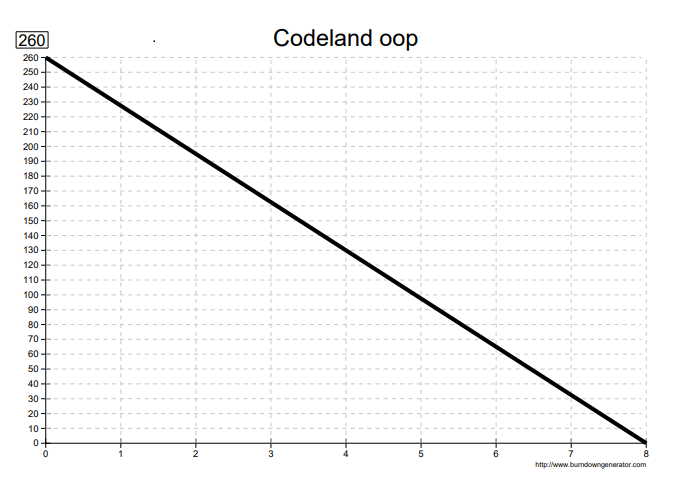
\includegraphics[scale=0.7]{img/quemado.png} 
		\caption{Grafica de quemado de las historias de usuario.}
		\label{quemado}
	\end{center}
\end{figure}